\problem{Масс-спектрометрия в органической химии}{8}

\ProblemPointsTwo{6}{4}{10}{8}

\hfill
\begin{minipage}{0.5\textwidth}
  \raggedleft
  Теория становится материальной силой, как только она овладевает массами.

  \textit{Карл Маркс.}\\
  \textit{К критике гегелевской философии права}
\end{minipage}

Суть масс-спектрометрического анализа заключается в переводе молекул образца в ионизированную форму с последующим разделением и регистрацией образующихся при этом положительных или отрицательных ионов.

Одним из важнейших преобразований ионов является перегруппировка
Мак-Лафферти. Она протекает благодаря миграции атома водорода
от $\gamma$-атома углерода через шестичленное переходное состояние:
\nopagebreak
\begin{figure}[H]
  \centering
  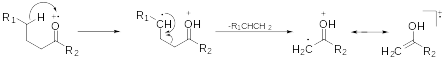
\includegraphics[width=0.9\textwidth]{problems/problem3/images/image1}
\end{figure}

\begin{enumerate}
  \item Для каких соединений произойдет перегруппировка Мак-Лафферти и для каких она будет подавлена? Ответ предоставьте схематически. Считайте, что катион-радикальный центр расположен на атоме кислорода.
  \nopagebreak
    \begin{enumerate}
      \item пентаналь
      \item гептен-5-он-2
      \item бутанон-2
      \item деканон-4
      \item октен-4-он-3
    \end{enumerate}

  \item Какому из изомерных соединений (пентаналь или 2-метилбутаналь) принадлежит указанный масс-спектр электронной ионизации? Ответ обоснуйте.
\end{enumerate}

\begin{minipage}{\textwidth}
  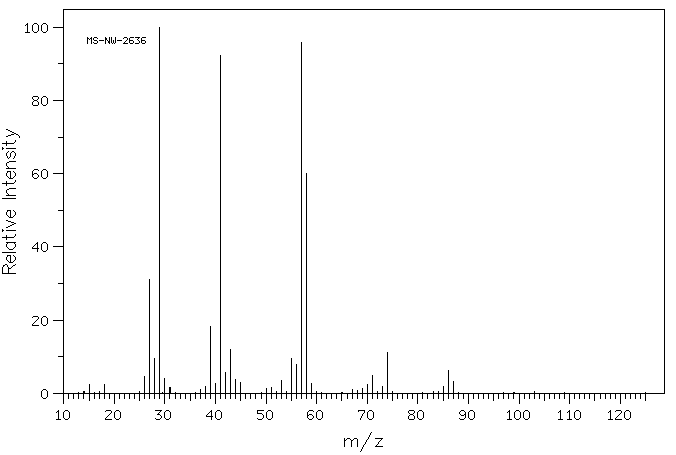
\includegraphics[width=0.65\textwidth]{problems/problem3/images/image2}
  \hspace{0.05\textwidth}
  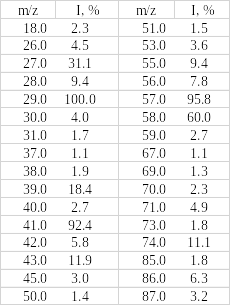
\includegraphics[width=0.3\textwidth]{problems/problem3/images/image3}
\end{minipage}
